% Created by tikzDevice version 0.12.3.1 on 2021-02-24 18:45:59
% !TEX encoding = UTF-8 Unicode
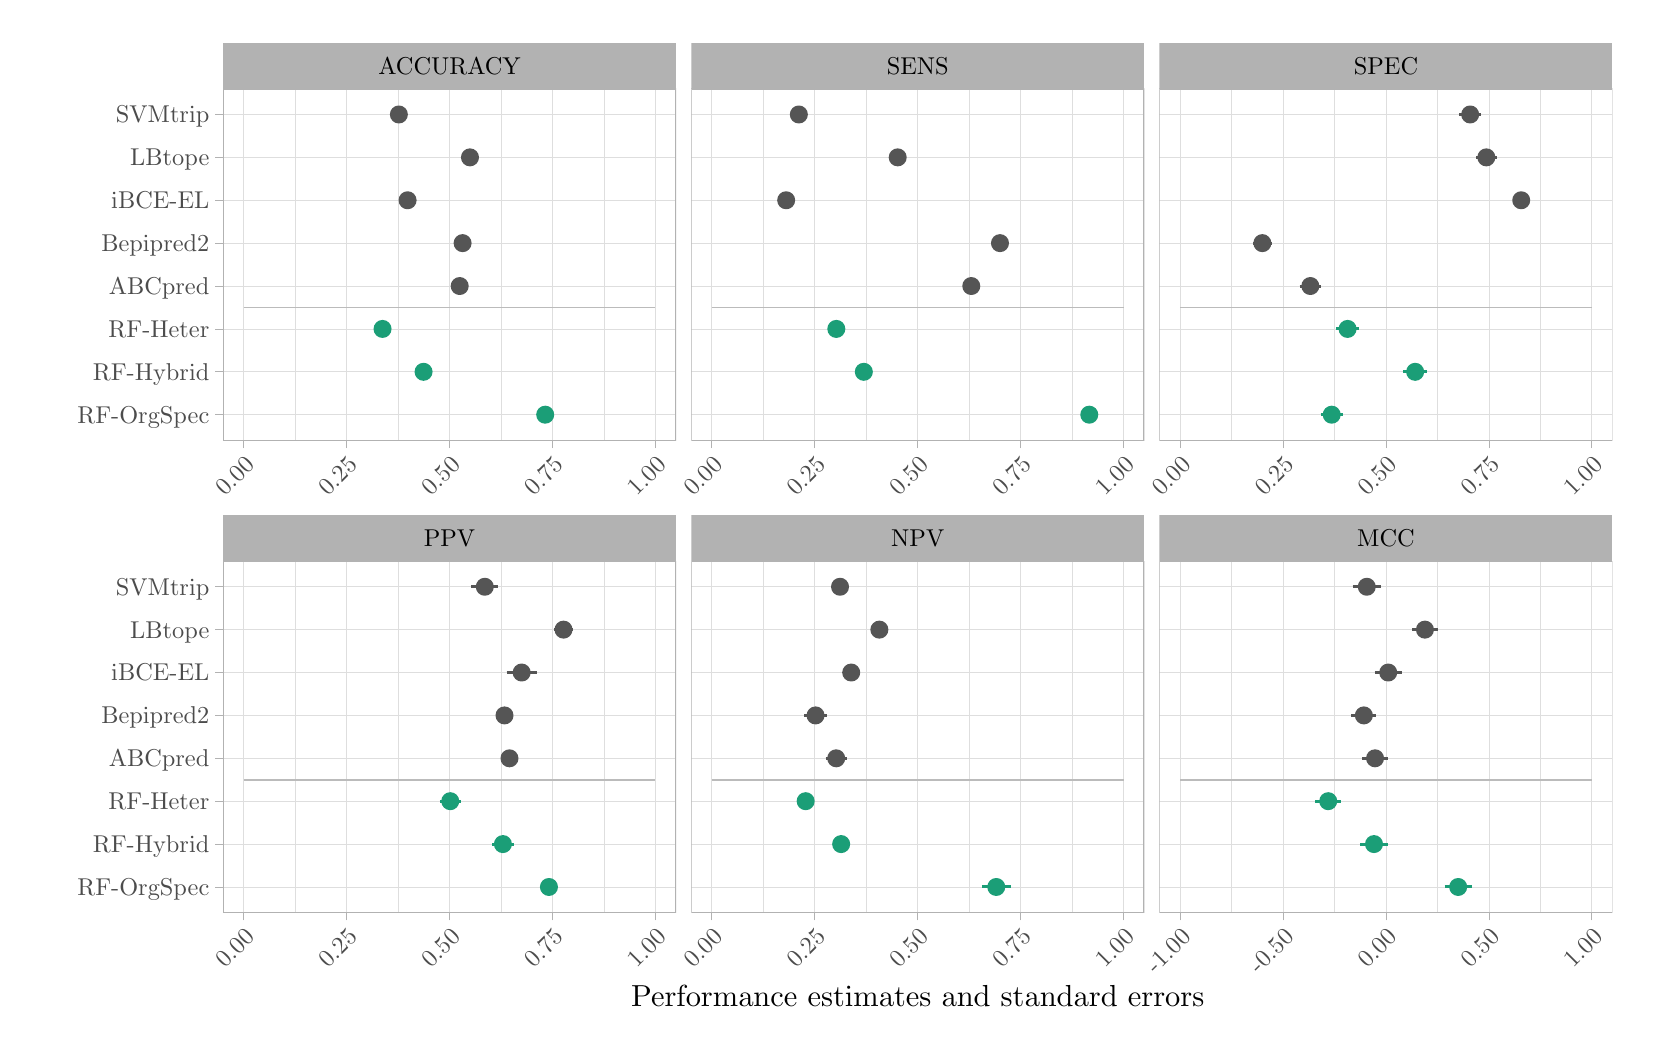
\begin{tikzpicture}[x=1pt,y=1pt]
\definecolor{fillColor}{RGB}{255,255,255}
\path[use as bounding box,fill=fillColor,fill opacity=0.00] (0,0) rectangle (578.16,361.35);
\begin{scope}
\path[clip] (  0.00,  0.00) rectangle (578.16,361.35);
\definecolor{drawColor}{RGB}{255,255,255}
\definecolor{fillColor}{RGB}{255,255,255}

\path[draw=drawColor,line width= 0.6pt,line join=round,line cap=round,fill=fillColor] (  0.00,  0.00) rectangle (578.16,361.35);
\end{scope}
\begin{scope}
\path[clip] ( 70.59,212.20) rectangle (234.28,339.28);
\definecolor{fillColor}{RGB}{255,255,255}

\path[fill=fillColor] ( 70.59,212.20) rectangle (234.28,339.28);
\definecolor{drawColor}{gray}{0.87}

\path[draw=drawColor,line width= 0.1pt,line join=round] ( 96.64,212.20) --
	( 96.64,339.28);

\path[draw=drawColor,line width= 0.1pt,line join=round] (133.84,212.20) --
	(133.84,339.28);

\path[draw=drawColor,line width= 0.1pt,line join=round] (171.04,212.20) --
	(171.04,339.28);

\path[draw=drawColor,line width= 0.1pt,line join=round] (208.24,212.20) --
	(208.24,339.28);

\path[draw=drawColor,line width= 0.3pt,line join=round] ( 70.59,221.50) --
	(234.28,221.50);

\path[draw=drawColor,line width= 0.3pt,line join=round] ( 70.59,236.99) --
	(234.28,236.99);

\path[draw=drawColor,line width= 0.3pt,line join=round] ( 70.59,252.49) --
	(234.28,252.49);

\path[draw=drawColor,line width= 0.3pt,line join=round] ( 70.59,267.99) --
	(234.28,267.99);

\path[draw=drawColor,line width= 0.3pt,line join=round] ( 70.59,283.49) --
	(234.28,283.49);

\path[draw=drawColor,line width= 0.3pt,line join=round] ( 70.59,298.98) --
	(234.28,298.98);

\path[draw=drawColor,line width= 0.3pt,line join=round] ( 70.59,314.48) --
	(234.28,314.48);

\path[draw=drawColor,line width= 0.3pt,line join=round] ( 70.59,329.98) --
	(234.28,329.98);

\path[draw=drawColor,line width= 0.3pt,line join=round] ( 78.03,212.20) --
	( 78.03,339.28);

\path[draw=drawColor,line width= 0.3pt,line join=round] (115.24,212.20) --
	(115.24,339.28);

\path[draw=drawColor,line width= 0.3pt,line join=round] (152.44,212.20) --
	(152.44,339.28);

\path[draw=drawColor,line width= 0.3pt,line join=round] (189.64,212.20) --
	(189.64,339.28);

\path[draw=drawColor,line width= 0.3pt,line join=round] (226.84,212.20) --
	(226.84,339.28);
\definecolor{drawColor}{RGB}{27,158,119}

\path[draw=drawColor,line width= 1.1pt,line join=round] (184.78,221.50) -- (189.25,221.50);

\path[draw=drawColor,line width= 1.1pt,line join=round] (140.60,236.99) -- (145.49,236.99);

\path[draw=drawColor,line width= 1.1pt,line join=round] (126.02,252.49) -- (130.44,252.49);
\definecolor{drawColor}{RGB}{85,85,85}

\path[draw=drawColor,line width= 1.1pt,line join=round] (153.79,267.99) -- (158.42,267.99);

\path[draw=drawColor,line width= 1.1pt,line join=round] (154.74,283.49) -- (159.58,283.49);

\path[draw=drawColor,line width= 1.1pt,line join=round] (134.86,298.98) -- (139.71,298.98);

\path[draw=drawColor,line width= 1.1pt,line join=round] (157.41,314.48) -- (162.22,314.48);

\path[draw=drawColor,line width= 1.1pt,line join=round] (131.71,329.98) -- (136.54,329.98);
\definecolor{drawColor}{RGB}{27,158,119}
\definecolor{fillColor}{RGB}{27,158,119}

\path[draw=drawColor,line width= 0.8pt,line join=round,line cap=round,fill=fillColor] (187.01,221.50) circle (  2.85);

\path[draw=drawColor,line width= 0.8pt,line join=round,line cap=round,fill=fillColor] (143.05,236.99) circle (  2.85);

\path[draw=drawColor,line width= 0.8pt,line join=round,line cap=round,fill=fillColor] (128.23,252.49) circle (  2.85);
\definecolor{drawColor}{RGB}{85,85,85}
\definecolor{fillColor}{RGB}{85,85,85}

\path[draw=drawColor,line width= 0.8pt,line join=round,line cap=round,fill=fillColor] (156.11,267.99) circle (  2.85);

\path[draw=drawColor,line width= 0.8pt,line join=round,line cap=round,fill=fillColor] (157.16,283.49) circle (  2.85);

\path[draw=drawColor,line width= 0.8pt,line join=round,line cap=round,fill=fillColor] (137.28,298.98) circle (  2.85);

\path[draw=drawColor,line width= 0.8pt,line join=round,line cap=round,fill=fillColor] (159.82,314.48) circle (  2.85);

\path[draw=drawColor,line width= 0.8pt,line join=round,line cap=round,fill=fillColor] (134.13,329.98) circle (  2.85);
\definecolor{drawColor}{RGB}{187,187,187}

\path[draw=drawColor,line width= 0.6pt,line join=round] ( 78.03,260.24) -- (226.84,260.24);
\definecolor{drawColor}{gray}{0.70}

\path[draw=drawColor,line width= 0.6pt,line join=round,line cap=round] ( 70.59,212.20) rectangle (234.28,339.28);
\end{scope}
\begin{scope}
\path[clip] ( 70.59, 41.54) rectangle (234.28,168.62);
\definecolor{fillColor}{RGB}{255,255,255}

\path[fill=fillColor] ( 70.59, 41.54) rectangle (234.28,168.62);
\definecolor{drawColor}{gray}{0.87}

\path[draw=drawColor,line width= 0.1pt,line join=round] ( 96.64, 41.54) --
	( 96.64,168.62);

\path[draw=drawColor,line width= 0.1pt,line join=round] (133.84, 41.54) --
	(133.84,168.62);

\path[draw=drawColor,line width= 0.1pt,line join=round] (171.04, 41.54) --
	(171.04,168.62);

\path[draw=drawColor,line width= 0.1pt,line join=round] (208.24, 41.54) --
	(208.24,168.62);

\path[draw=drawColor,line width= 0.3pt,line join=round] ( 70.59, 50.84) --
	(234.28, 50.84);

\path[draw=drawColor,line width= 0.3pt,line join=round] ( 70.59, 66.34) --
	(234.28, 66.34);

\path[draw=drawColor,line width= 0.3pt,line join=round] ( 70.59, 81.84) --
	(234.28, 81.84);

\path[draw=drawColor,line width= 0.3pt,line join=round] ( 70.59, 97.33) --
	(234.28, 97.33);

\path[draw=drawColor,line width= 0.3pt,line join=round] ( 70.59,112.83) --
	(234.28,112.83);

\path[draw=drawColor,line width= 0.3pt,line join=round] ( 70.59,128.33) --
	(234.28,128.33);

\path[draw=drawColor,line width= 0.3pt,line join=round] ( 70.59,143.83) --
	(234.28,143.83);

\path[draw=drawColor,line width= 0.3pt,line join=round] ( 70.59,159.32) --
	(234.28,159.32);

\path[draw=drawColor,line width= 0.3pt,line join=round] ( 78.03, 41.54) --
	( 78.03,168.62);

\path[draw=drawColor,line width= 0.3pt,line join=round] (115.24, 41.54) --
	(115.24,168.62);

\path[draw=drawColor,line width= 0.3pt,line join=round] (152.44, 41.54) --
	(152.44,168.62);

\path[draw=drawColor,line width= 0.3pt,line join=round] (189.64, 41.54) --
	(189.64,168.62);

\path[draw=drawColor,line width= 0.3pt,line join=round] (226.84, 41.54) --
	(226.84,168.62);
\definecolor{drawColor}{RGB}{27,158,119}

\path[draw=drawColor,line width= 1.1pt,line join=round] (185.95, 50.84) -- (190.78, 50.84);

\path[draw=drawColor,line width= 1.1pt,line join=round] (167.84, 66.34) -- (175.62, 66.34);

\path[draw=drawColor,line width= 1.1pt,line join=round] (148.93, 81.84) -- (156.48, 81.84);
\definecolor{drawColor}{RGB}{85,85,85}

\path[draw=drawColor,line width= 1.1pt,line join=round] (171.23, 97.33) -- (176.98, 97.33);

\path[draw=drawColor,line width= 1.1pt,line join=round] (169.49,112.83) -- (175.11,112.83);

\path[draw=drawColor,line width= 1.1pt,line join=round] (173.05,128.33) -- (183.95,128.33);

\path[draw=drawColor,line width= 1.1pt,line join=round] (190.26,143.83) -- (197.01,143.83);

\path[draw=drawColor,line width= 1.1pt,line join=round] (160.25,159.32) -- (170.11,159.32);
\definecolor{drawColor}{RGB}{27,158,119}
\definecolor{fillColor}{RGB}{27,158,119}

\path[draw=drawColor,line width= 0.8pt,line join=round,line cap=round,fill=fillColor] (188.36, 50.84) circle (  2.85);

\path[draw=drawColor,line width= 0.8pt,line join=round,line cap=round,fill=fillColor] (171.73, 66.34) circle (  2.85);

\path[draw=drawColor,line width= 0.8pt,line join=round,line cap=round,fill=fillColor] (152.70, 81.84) circle (  2.85);
\definecolor{drawColor}{RGB}{85,85,85}
\definecolor{fillColor}{RGB}{85,85,85}

\path[draw=drawColor,line width= 0.8pt,line join=round,line cap=round,fill=fillColor] (174.10, 97.33) circle (  2.85);

\path[draw=drawColor,line width= 0.8pt,line join=round,line cap=round,fill=fillColor] (172.30,112.83) circle (  2.85);

\path[draw=drawColor,line width= 0.8pt,line join=round,line cap=round,fill=fillColor] (178.50,128.33) circle (  2.85);

\path[draw=drawColor,line width= 0.8pt,line join=round,line cap=round,fill=fillColor] (193.63,143.83) circle (  2.85);

\path[draw=drawColor,line width= 0.8pt,line join=round,line cap=round,fill=fillColor] (165.18,159.32) circle (  2.85);
\definecolor{drawColor}{RGB}{187,187,187}

\path[draw=drawColor,line width= 0.6pt,line join=round] ( 78.03, 89.59) -- (226.84, 89.59);
\definecolor{drawColor}{gray}{0.70}

\path[draw=drawColor,line width= 0.6pt,line join=round,line cap=round] ( 70.59, 41.54) rectangle (234.28,168.62);
\end{scope}
\begin{scope}
\path[clip] (239.78,212.20) rectangle (403.47,339.28);
\definecolor{fillColor}{RGB}{255,255,255}

\path[fill=fillColor] (239.78,212.20) rectangle (403.47,339.28);
\definecolor{drawColor}{gray}{0.87}

\path[draw=drawColor,line width= 0.1pt,line join=round] (265.82,212.20) --
	(265.82,339.28);

\path[draw=drawColor,line width= 0.1pt,line join=round] (303.03,212.20) --
	(303.03,339.28);

\path[draw=drawColor,line width= 0.1pt,line join=round] (340.23,212.20) --
	(340.23,339.28);

\path[draw=drawColor,line width= 0.1pt,line join=round] (377.43,212.20) --
	(377.43,339.28);

\path[draw=drawColor,line width= 0.3pt,line join=round] (239.78,221.50) --
	(403.47,221.50);

\path[draw=drawColor,line width= 0.3pt,line join=round] (239.78,236.99) --
	(403.47,236.99);

\path[draw=drawColor,line width= 0.3pt,line join=round] (239.78,252.49) --
	(403.47,252.49);

\path[draw=drawColor,line width= 0.3pt,line join=round] (239.78,267.99) --
	(403.47,267.99);

\path[draw=drawColor,line width= 0.3pt,line join=round] (239.78,283.49) --
	(403.47,283.49);

\path[draw=drawColor,line width= 0.3pt,line join=round] (239.78,298.98) --
	(403.47,298.98);

\path[draw=drawColor,line width= 0.3pt,line join=round] (239.78,314.48) --
	(403.47,314.48);

\path[draw=drawColor,line width= 0.3pt,line join=round] (239.78,329.98) --
	(403.47,329.98);

\path[draw=drawColor,line width= 0.3pt,line join=round] (247.22,212.20) --
	(247.22,339.28);

\path[draw=drawColor,line width= 0.3pt,line join=round] (284.43,212.20) --
	(284.43,339.28);

\path[draw=drawColor,line width= 0.3pt,line join=round] (321.63,212.20) --
	(321.63,339.28);

\path[draw=drawColor,line width= 0.3pt,line join=round] (358.83,212.20) --
	(358.83,339.28);

\path[draw=drawColor,line width= 0.3pt,line join=round] (396.03,212.20) --
	(396.03,339.28);
\definecolor{drawColor}{RGB}{27,158,119}

\path[draw=drawColor,line width= 1.1pt,line join=round] (381.96,221.50) -- (385.26,221.50);

\path[draw=drawColor,line width= 1.1pt,line join=round] (299.28,236.99) -- (305.01,236.99);

\path[draw=drawColor,line width= 1.1pt,line join=round] (289.60,252.49) -- (294.80,252.49);
\definecolor{drawColor}{RGB}{85,85,85}

\path[draw=drawColor,line width= 1.1pt,line join=round] (338.20,267.99) -- (343.75,267.99);

\path[draw=drawColor,line width= 1.1pt,line join=round] (348.65,283.49) -- (354.03,283.49);

\path[draw=drawColor,line width= 1.1pt,line join=round] (271.77,298.98) -- (276.38,298.98);

\path[draw=drawColor,line width= 1.1pt,line join=round] (311.40,314.48) -- (317.36,314.48);

\path[draw=drawColor,line width= 1.1pt,line join=round] (276.29,329.98) -- (281.03,329.98);
\definecolor{drawColor}{RGB}{27,158,119}
\definecolor{fillColor}{RGB}{27,158,119}

\path[draw=drawColor,line width= 0.8pt,line join=round,line cap=round,fill=fillColor] (383.61,221.50) circle (  2.85);

\path[draw=drawColor,line width= 0.8pt,line join=round,line cap=round,fill=fillColor] (302.14,236.99) circle (  2.85);

\path[draw=drawColor,line width= 0.8pt,line join=round,line cap=round,fill=fillColor] (292.20,252.49) circle (  2.85);
\definecolor{drawColor}{RGB}{85,85,85}
\definecolor{fillColor}{RGB}{85,85,85}

\path[draw=drawColor,line width= 0.8pt,line join=round,line cap=round,fill=fillColor] (340.97,267.99) circle (  2.85);

\path[draw=drawColor,line width= 0.8pt,line join=round,line cap=round,fill=fillColor] (351.34,283.49) circle (  2.85);

\path[draw=drawColor,line width= 0.8pt,line join=round,line cap=round,fill=fillColor] (274.08,298.98) circle (  2.85);

\path[draw=drawColor,line width= 0.8pt,line join=round,line cap=round,fill=fillColor] (314.38,314.48) circle (  2.85);

\path[draw=drawColor,line width= 0.8pt,line join=round,line cap=round,fill=fillColor] (278.66,329.98) circle (  2.85);
\definecolor{drawColor}{RGB}{187,187,187}

\path[draw=drawColor,line width= 0.6pt,line join=round] (247.22,260.24) -- (396.03,260.24);
\definecolor{drawColor}{gray}{0.70}

\path[draw=drawColor,line width= 0.6pt,line join=round,line cap=round] (239.78,212.20) rectangle (403.47,339.28);
\end{scope}
\begin{scope}
\path[clip] (239.78, 41.54) rectangle (403.47,168.62);
\definecolor{fillColor}{RGB}{255,255,255}

\path[fill=fillColor] (239.78, 41.54) rectangle (403.47,168.62);
\definecolor{drawColor}{gray}{0.87}

\path[draw=drawColor,line width= 0.1pt,line join=round] (265.82, 41.54) --
	(265.82,168.62);

\path[draw=drawColor,line width= 0.1pt,line join=round] (303.03, 41.54) --
	(303.03,168.62);

\path[draw=drawColor,line width= 0.1pt,line join=round] (340.23, 41.54) --
	(340.23,168.62);

\path[draw=drawColor,line width= 0.1pt,line join=round] (377.43, 41.54) --
	(377.43,168.62);

\path[draw=drawColor,line width= 0.3pt,line join=round] (239.78, 50.84) --
	(403.47, 50.84);

\path[draw=drawColor,line width= 0.3pt,line join=round] (239.78, 66.34) --
	(403.47, 66.34);

\path[draw=drawColor,line width= 0.3pt,line join=round] (239.78, 81.84) --
	(403.47, 81.84);

\path[draw=drawColor,line width= 0.3pt,line join=round] (239.78, 97.33) --
	(403.47, 97.33);

\path[draw=drawColor,line width= 0.3pt,line join=round] (239.78,112.83) --
	(403.47,112.83);

\path[draw=drawColor,line width= 0.3pt,line join=round] (239.78,128.33) --
	(403.47,128.33);

\path[draw=drawColor,line width= 0.3pt,line join=round] (239.78,143.83) --
	(403.47,143.83);

\path[draw=drawColor,line width= 0.3pt,line join=round] (239.78,159.32) --
	(403.47,159.32);

\path[draw=drawColor,line width= 0.3pt,line join=round] (247.22, 41.54) --
	(247.22,168.62);

\path[draw=drawColor,line width= 0.3pt,line join=round] (284.43, 41.54) --
	(284.43,168.62);

\path[draw=drawColor,line width= 0.3pt,line join=round] (321.63, 41.54) --
	(321.63,168.62);

\path[draw=drawColor,line width= 0.3pt,line join=round] (358.83, 41.54) --
	(358.83,168.62);

\path[draw=drawColor,line width= 0.3pt,line join=round] (396.03, 41.54) --
	(396.03,168.62);
\definecolor{drawColor}{RGB}{27,158,119}

\path[draw=drawColor,line width= 1.1pt,line join=round] (344.76, 50.84) -- (355.25, 50.84);

\path[draw=drawColor,line width= 1.1pt,line join=round] (290.99, 66.34) -- (296.92, 66.34);

\path[draw=drawColor,line width= 1.1pt,line join=round] (278.49, 81.84) -- (283.75, 81.84);
\definecolor{drawColor}{RGB}{85,85,85}

\path[draw=drawColor,line width= 1.1pt,line join=round] (288.37, 97.33) -- (295.95, 97.33);

\path[draw=drawColor,line width= 1.1pt,line join=round] (280.65,112.83) -- (288.75,112.83);

\path[draw=drawColor,line width= 1.1pt,line join=round] (294.97,128.33) -- (300.19,128.33);

\path[draw=drawColor,line width= 1.1pt,line join=round] (304.71,143.83) -- (310.81,143.83);

\path[draw=drawColor,line width= 1.1pt,line join=round] (290.86,159.32) -- (296.21,159.32);
\definecolor{drawColor}{RGB}{27,158,119}
\definecolor{fillColor}{RGB}{27,158,119}

\path[draw=drawColor,line width= 0.8pt,line join=round,line cap=round,fill=fillColor] (350.00, 50.84) circle (  2.85);

\path[draw=drawColor,line width= 0.8pt,line join=round,line cap=round,fill=fillColor] (293.95, 66.34) circle (  2.85);

\path[draw=drawColor,line width= 0.8pt,line join=round,line cap=round,fill=fillColor] (281.12, 81.84) circle (  2.85);
\definecolor{drawColor}{RGB}{85,85,85}
\definecolor{fillColor}{RGB}{85,85,85}

\path[draw=drawColor,line width= 0.8pt,line join=round,line cap=round,fill=fillColor] (292.16, 97.33) circle (  2.85);

\path[draw=drawColor,line width= 0.8pt,line join=round,line cap=round,fill=fillColor] (284.70,112.83) circle (  2.85);

\path[draw=drawColor,line width= 0.8pt,line join=round,line cap=round,fill=fillColor] (297.58,128.33) circle (  2.85);

\path[draw=drawColor,line width= 0.8pt,line join=round,line cap=round,fill=fillColor] (307.76,143.83) circle (  2.85);

\path[draw=drawColor,line width= 0.8pt,line join=round,line cap=round,fill=fillColor] (293.54,159.32) circle (  2.85);
\definecolor{drawColor}{RGB}{187,187,187}

\path[draw=drawColor,line width= 0.6pt,line join=round] (247.22, 89.59) -- (396.03, 89.59);
\definecolor{drawColor}{gray}{0.70}

\path[draw=drawColor,line width= 0.6pt,line join=round,line cap=round] (239.78, 41.54) rectangle (403.47,168.62);
\end{scope}
\begin{scope}
\path[clip] (408.97,212.20) rectangle (572.66,339.28);
\definecolor{fillColor}{RGB}{255,255,255}

\path[fill=fillColor] (408.97,212.20) rectangle (572.66,339.28);
\definecolor{drawColor}{gray}{0.87}

\path[draw=drawColor,line width= 0.1pt,line join=round] (435.01,212.20) --
	(435.01,339.28);

\path[draw=drawColor,line width= 0.1pt,line join=round] (472.21,212.20) --
	(472.21,339.28);

\path[draw=drawColor,line width= 0.1pt,line join=round] (509.42,212.20) --
	(509.42,339.28);

\path[draw=drawColor,line width= 0.1pt,line join=round] (546.62,212.20) --
	(546.62,339.28);

\path[draw=drawColor,line width= 0.3pt,line join=round] (408.97,221.50) --
	(572.66,221.50);

\path[draw=drawColor,line width= 0.3pt,line join=round] (408.97,236.99) --
	(572.66,236.99);

\path[draw=drawColor,line width= 0.3pt,line join=round] (408.97,252.49) --
	(572.66,252.49);

\path[draw=drawColor,line width= 0.3pt,line join=round] (408.97,267.99) --
	(572.66,267.99);

\path[draw=drawColor,line width= 0.3pt,line join=round] (408.97,283.49) --
	(572.66,283.49);

\path[draw=drawColor,line width= 0.3pt,line join=round] (408.97,298.98) --
	(572.66,298.98);

\path[draw=drawColor,line width= 0.3pt,line join=round] (408.97,314.48) --
	(572.66,314.48);

\path[draw=drawColor,line width= 0.3pt,line join=round] (408.97,329.98) --
	(572.66,329.98);

\path[draw=drawColor,line width= 0.3pt,line join=round] (416.41,212.20) --
	(416.41,339.28);

\path[draw=drawColor,line width= 0.3pt,line join=round] (453.61,212.20) --
	(453.61,339.28);

\path[draw=drawColor,line width= 0.3pt,line join=round] (490.82,212.20) --
	(490.82,339.28);

\path[draw=drawColor,line width= 0.3pt,line join=round] (528.02,212.20) --
	(528.02,339.28);

\path[draw=drawColor,line width= 0.3pt,line join=round] (565.22,212.20) --
	(565.22,339.28);
\definecolor{drawColor}{RGB}{27,158,119}

\path[draw=drawColor,line width= 1.1pt,line join=round] (467.16,221.50) -- (475.27,221.50);

\path[draw=drawColor,line width= 1.1pt,line join=round] (497.07,236.99) -- (505.66,236.99);

\path[draw=drawColor,line width= 1.1pt,line join=round] (472.92,252.49) -- (480.97,252.49);
\definecolor{drawColor}{RGB}{85,85,85}

\path[draw=drawColor,line width= 1.1pt,line join=round] (459.57,267.99) -- (467.41,267.99);

\path[draw=drawColor,line width= 1.1pt,line join=round] (442.83,283.49) -- (449.46,283.49);

\path[draw=drawColor,line width= 1.1pt,line join=round] (536.54,298.98) -- (542.83,298.98);

\path[draw=drawColor,line width= 1.1pt,line join=round] (523.35,314.48) -- (530.84,314.48);

\path[draw=drawColor,line width= 1.1pt,line join=round] (517.32,329.98) -- (525.15,329.98);
\definecolor{drawColor}{RGB}{27,158,119}
\definecolor{fillColor}{RGB}{27,158,119}

\path[draw=drawColor,line width= 0.8pt,line join=round,line cap=round,fill=fillColor] (471.21,221.50) circle (  2.85);

\path[draw=drawColor,line width= 0.8pt,line join=round,line cap=round,fill=fillColor] (501.36,236.99) circle (  2.85);

\path[draw=drawColor,line width= 0.8pt,line join=round,line cap=round,fill=fillColor] (476.94,252.49) circle (  2.85);
\definecolor{drawColor}{RGB}{85,85,85}
\definecolor{fillColor}{RGB}{85,85,85}

\path[draw=drawColor,line width= 0.8pt,line join=round,line cap=round,fill=fillColor] (463.49,267.99) circle (  2.85);

\path[draw=drawColor,line width= 0.8pt,line join=round,line cap=round,fill=fillColor] (446.15,283.49) circle (  2.85);

\path[draw=drawColor,line width= 0.8pt,line join=round,line cap=round,fill=fillColor] (539.69,298.98) circle (  2.85);

\path[draw=drawColor,line width= 0.8pt,line join=round,line cap=round,fill=fillColor] (527.09,314.48) circle (  2.85);

\path[draw=drawColor,line width= 0.8pt,line join=round,line cap=round,fill=fillColor] (521.24,329.98) circle (  2.85);
\definecolor{drawColor}{RGB}{187,187,187}

\path[draw=drawColor,line width= 0.6pt,line join=round] (416.41,260.24) -- (565.22,260.24);
\definecolor{drawColor}{gray}{0.70}

\path[draw=drawColor,line width= 0.6pt,line join=round,line cap=round] (408.97,212.20) rectangle (572.66,339.28);
\end{scope}
\begin{scope}
\path[clip] (408.97, 41.54) rectangle (572.66,168.62);
\definecolor{fillColor}{RGB}{255,255,255}

\path[fill=fillColor] (408.97, 41.54) rectangle (572.66,168.62);
\definecolor{drawColor}{gray}{0.87}

\path[draw=drawColor,line width= 0.1pt,line join=round] (435.01, 41.54) --
	(435.01,168.62);

\path[draw=drawColor,line width= 0.1pt,line join=round] (472.21, 41.54) --
	(472.21,168.62);

\path[draw=drawColor,line width= 0.1pt,line join=round] (509.42, 41.54) --
	(509.42,168.62);

\path[draw=drawColor,line width= 0.1pt,line join=round] (546.62, 41.54) --
	(546.62,168.62);

\path[draw=drawColor,line width= 0.3pt,line join=round] (408.97, 50.84) --
	(572.66, 50.84);

\path[draw=drawColor,line width= 0.3pt,line join=round] (408.97, 66.34) --
	(572.66, 66.34);

\path[draw=drawColor,line width= 0.3pt,line join=round] (408.97, 81.84) --
	(572.66, 81.84);

\path[draw=drawColor,line width= 0.3pt,line join=round] (408.97, 97.33) --
	(572.66, 97.33);

\path[draw=drawColor,line width= 0.3pt,line join=round] (408.97,112.83) --
	(572.66,112.83);

\path[draw=drawColor,line width= 0.3pt,line join=round] (408.97,128.33) --
	(572.66,128.33);

\path[draw=drawColor,line width= 0.3pt,line join=round] (408.97,143.83) --
	(572.66,143.83);

\path[draw=drawColor,line width= 0.3pt,line join=round] (408.97,159.32) --
	(572.66,159.32);

\path[draw=drawColor,line width= 0.3pt,line join=round] (416.41, 41.54) --
	(416.41,168.62);

\path[draw=drawColor,line width= 0.3pt,line join=round] (453.61, 41.54) --
	(453.61,168.62);

\path[draw=drawColor,line width= 0.3pt,line join=round] (490.82, 41.54) --
	(490.82,168.62);

\path[draw=drawColor,line width= 0.3pt,line join=round] (528.02, 41.54) --
	(528.02,168.62);

\path[draw=drawColor,line width= 0.3pt,line join=round] (565.22, 41.54) --
	(565.22,168.62);
\definecolor{drawColor}{RGB}{27,158,119}

\path[draw=drawColor,line width= 1.1pt,line join=round] (512.00, 50.84) -- (521.82, 50.84);

\path[draw=drawColor,line width= 1.1pt,line join=round] (481.45, 66.34) -- (491.52, 66.34);

\path[draw=drawColor,line width= 1.1pt,line join=round] (465.33, 81.84) -- (474.56, 81.84);
\definecolor{drawColor}{RGB}{85,85,85}

\path[draw=drawColor,line width= 1.1pt,line join=round] (482.23, 97.33) -- (491.51, 97.33);

\path[draw=drawColor,line width= 1.1pt,line join=round] (478.29,112.83) -- (487.37,112.83);

\path[draw=drawColor,line width= 1.1pt,line join=round] (486.80,128.33) -- (496.46,128.33);

\path[draw=drawColor,line width= 1.1pt,line join=round] (500.31,143.83) -- (509.49,143.83);

\path[draw=drawColor,line width= 1.1pt,line join=round] (478.79,159.32) -- (488.96,159.32);
\definecolor{drawColor}{RGB}{27,158,119}
\definecolor{fillColor}{RGB}{27,158,119}

\path[draw=drawColor,line width= 0.8pt,line join=round,line cap=round,fill=fillColor] (516.91, 50.84) circle (  2.85);

\path[draw=drawColor,line width= 0.8pt,line join=round,line cap=round,fill=fillColor] (486.49, 66.34) circle (  2.85);

\path[draw=drawColor,line width= 0.8pt,line join=round,line cap=round,fill=fillColor] (469.95, 81.84) circle (  2.85);
\definecolor{drawColor}{RGB}{85,85,85}
\definecolor{fillColor}{RGB}{85,85,85}

\path[draw=drawColor,line width= 0.8pt,line join=round,line cap=round,fill=fillColor] (486.87, 97.33) circle (  2.85);

\path[draw=drawColor,line width= 0.8pt,line join=round,line cap=round,fill=fillColor] (482.83,112.83) circle (  2.85);

\path[draw=drawColor,line width= 0.8pt,line join=round,line cap=round,fill=fillColor] (491.63,128.33) circle (  2.85);

\path[draw=drawColor,line width= 0.8pt,line join=round,line cap=round,fill=fillColor] (504.90,143.83) circle (  2.85);

\path[draw=drawColor,line width= 0.8pt,line join=round,line cap=round,fill=fillColor] (483.88,159.32) circle (  2.85);
\definecolor{drawColor}{RGB}{187,187,187}

\path[draw=drawColor,line width= 0.6pt,line join=round] (416.41, 89.59) -- (565.22, 89.59);
\definecolor{drawColor}{gray}{0.70}

\path[draw=drawColor,line width= 0.6pt,line join=round,line cap=round] (408.97, 41.54) rectangle (572.66,168.62);
\end{scope}
\begin{scope}
\path[clip] ( 70.59,168.62) rectangle (234.28,185.19);
\definecolor{fillColor}{gray}{0.70}

\path[fill=fillColor] ( 70.59,168.62) rectangle (234.28,185.19);
\definecolor{drawColor}{RGB}{0,0,0}

\node[text=drawColor,anchor=base,inner sep=0pt, outer sep=0pt, scale=  0.88] at (152.44,173.88) {PPV};
\end{scope}
\begin{scope}
\path[clip] (239.78,168.62) rectangle (403.47,185.19);
\definecolor{fillColor}{gray}{0.70}

\path[fill=fillColor] (239.78,168.62) rectangle (403.47,185.19);
\definecolor{drawColor}{RGB}{0,0,0}

\node[text=drawColor,anchor=base,inner sep=0pt, outer sep=0pt, scale=  0.88] at (321.63,173.88) {NPV};
\end{scope}
\begin{scope}
\path[clip] (408.97,168.62) rectangle (572.66,185.19);
\definecolor{fillColor}{gray}{0.70}

\path[fill=fillColor] (408.97,168.62) rectangle (572.66,185.19);
\definecolor{drawColor}{RGB}{0,0,0}

\node[text=drawColor,anchor=base,inner sep=0pt, outer sep=0pt, scale=  0.88] at (490.82,173.88) {MCC};
\end{scope}
\begin{scope}
\path[clip] ( 70.59,339.28) rectangle (234.28,355.85);
\definecolor{fillColor}{gray}{0.70}

\path[fill=fillColor] ( 70.59,339.28) rectangle (234.28,355.85);
\definecolor{drawColor}{RGB}{0,0,0}

\node[text=drawColor,anchor=base,inner sep=0pt, outer sep=0pt, scale=  0.88] at (152.44,344.53) {ACCURACY};
\end{scope}
\begin{scope}
\path[clip] (239.78,339.28) rectangle (403.47,355.85);
\definecolor{fillColor}{gray}{0.70}

\path[fill=fillColor] (239.78,339.28) rectangle (403.47,355.85);
\definecolor{drawColor}{RGB}{0,0,0}

\node[text=drawColor,anchor=base,inner sep=0pt, outer sep=0pt, scale=  0.88] at (321.63,344.53) {SENS};
\end{scope}
\begin{scope}
\path[clip] (408.97,339.28) rectangle (572.66,355.85);
\definecolor{fillColor}{gray}{0.70}

\path[fill=fillColor] (408.97,339.28) rectangle (572.66,355.85);
\definecolor{drawColor}{RGB}{0,0,0}

\node[text=drawColor,anchor=base,inner sep=0pt, outer sep=0pt, scale=  0.88] at (490.82,344.53) {SPEC};
\end{scope}
\begin{scope}
\path[clip] (  0.00,  0.00) rectangle (578.16,361.35);
\definecolor{drawColor}{gray}{0.70}

\path[draw=drawColor,line width= 0.3pt,line join=round] ( 78.03, 38.79) --
	( 78.03, 41.54);

\path[draw=drawColor,line width= 0.3pt,line join=round] (115.24, 38.79) --
	(115.24, 41.54);

\path[draw=drawColor,line width= 0.3pt,line join=round] (152.44, 38.79) --
	(152.44, 41.54);

\path[draw=drawColor,line width= 0.3pt,line join=round] (189.64, 38.79) --
	(189.64, 41.54);

\path[draw=drawColor,line width= 0.3pt,line join=round] (226.84, 38.79) --
	(226.84, 41.54);
\end{scope}
\begin{scope}
\path[clip] (  0.00,  0.00) rectangle (578.16,361.35);
\definecolor{drawColor}{gray}{0.30}

\node[text=drawColor,rotate= 45.00,anchor=base east,inner sep=0pt, outer sep=0pt, scale=  0.88] at ( 82.32, 32.31) {0.00};

\node[text=drawColor,rotate= 45.00,anchor=base east,inner sep=0pt, outer sep=0pt, scale=  0.88] at (119.52, 32.31) {0.25};

\node[text=drawColor,rotate= 45.00,anchor=base east,inner sep=0pt, outer sep=0pt, scale=  0.88] at (156.72, 32.31) {0.50};

\node[text=drawColor,rotate= 45.00,anchor=base east,inner sep=0pt, outer sep=0pt, scale=  0.88] at (193.93, 32.31) {0.75};

\node[text=drawColor,rotate= 45.00,anchor=base east,inner sep=0pt, outer sep=0pt, scale=  0.88] at (231.13, 32.31) {1.00};
\end{scope}
\begin{scope}
\path[clip] (  0.00,  0.00) rectangle (578.16,361.35);
\definecolor{drawColor}{gray}{0.70}

\path[draw=drawColor,line width= 0.3pt,line join=round] (247.22, 38.79) --
	(247.22, 41.54);

\path[draw=drawColor,line width= 0.3pt,line join=round] (284.43, 38.79) --
	(284.43, 41.54);

\path[draw=drawColor,line width= 0.3pt,line join=round] (321.63, 38.79) --
	(321.63, 41.54);

\path[draw=drawColor,line width= 0.3pt,line join=round] (358.83, 38.79) --
	(358.83, 41.54);

\path[draw=drawColor,line width= 0.3pt,line join=round] (396.03, 38.79) --
	(396.03, 41.54);
\end{scope}
\begin{scope}
\path[clip] (  0.00,  0.00) rectangle (578.16,361.35);
\definecolor{drawColor}{gray}{0.30}

\node[text=drawColor,rotate= 45.00,anchor=base east,inner sep=0pt, outer sep=0pt, scale=  0.88] at (251.51, 32.31) {0.00};

\node[text=drawColor,rotate= 45.00,anchor=base east,inner sep=0pt, outer sep=0pt, scale=  0.88] at (288.71, 32.31) {0.25};

\node[text=drawColor,rotate= 45.00,anchor=base east,inner sep=0pt, outer sep=0pt, scale=  0.88] at (325.91, 32.31) {0.50};

\node[text=drawColor,rotate= 45.00,anchor=base east,inner sep=0pt, outer sep=0pt, scale=  0.88] at (363.11, 32.31) {0.75};

\node[text=drawColor,rotate= 45.00,anchor=base east,inner sep=0pt, outer sep=0pt, scale=  0.88] at (400.32, 32.31) {1.00};
\end{scope}
\begin{scope}
\path[clip] (  0.00,  0.00) rectangle (578.16,361.35);
\definecolor{drawColor}{gray}{0.70}

\path[draw=drawColor,line width= 0.3pt,line join=round] (416.41, 38.79) --
	(416.41, 41.54);

\path[draw=drawColor,line width= 0.3pt,line join=round] (453.61, 38.79) --
	(453.61, 41.54);

\path[draw=drawColor,line width= 0.3pt,line join=round] (490.82, 38.79) --
	(490.82, 41.54);

\path[draw=drawColor,line width= 0.3pt,line join=round] (528.02, 38.79) --
	(528.02, 41.54);

\path[draw=drawColor,line width= 0.3pt,line join=round] (565.22, 38.79) --
	(565.22, 41.54);
\end{scope}
\begin{scope}
\path[clip] (  0.00,  0.00) rectangle (578.16,361.35);
\definecolor{drawColor}{gray}{0.30}

\node[text=drawColor,rotate= 45.00,anchor=base east,inner sep=0pt, outer sep=0pt, scale=  0.88] at (420.70, 32.31) {-1.00};

\node[text=drawColor,rotate= 45.00,anchor=base east,inner sep=0pt, outer sep=0pt, scale=  0.88] at (457.90, 32.31) {-0.50};

\node[text=drawColor,rotate= 45.00,anchor=base east,inner sep=0pt, outer sep=0pt, scale=  0.88] at (495.10, 32.31) {0.00};

\node[text=drawColor,rotate= 45.00,anchor=base east,inner sep=0pt, outer sep=0pt, scale=  0.88] at (532.30, 32.31) {0.50};

\node[text=drawColor,rotate= 45.00,anchor=base east,inner sep=0pt, outer sep=0pt, scale=  0.88] at (569.51, 32.31) {1.00};
\end{scope}
\begin{scope}
\path[clip] (  0.00,  0.00) rectangle (578.16,361.35);
\definecolor{drawColor}{gray}{0.70}

\path[draw=drawColor,line width= 0.3pt,line join=round] ( 78.03,209.45) --
	( 78.03,212.20);

\path[draw=drawColor,line width= 0.3pt,line join=round] (115.24,209.45) --
	(115.24,212.20);

\path[draw=drawColor,line width= 0.3pt,line join=round] (152.44,209.45) --
	(152.44,212.20);

\path[draw=drawColor,line width= 0.3pt,line join=round] (189.64,209.45) --
	(189.64,212.20);

\path[draw=drawColor,line width= 0.3pt,line join=round] (226.84,209.45) --
	(226.84,212.20);
\end{scope}
\begin{scope}
\path[clip] (  0.00,  0.00) rectangle (578.16,361.35);
\definecolor{drawColor}{gray}{0.30}

\node[text=drawColor,rotate= 45.00,anchor=base east,inner sep=0pt, outer sep=0pt, scale=  0.88] at ( 82.32,202.96) {0.00};

\node[text=drawColor,rotate= 45.00,anchor=base east,inner sep=0pt, outer sep=0pt, scale=  0.88] at (119.52,202.96) {0.25};

\node[text=drawColor,rotate= 45.00,anchor=base east,inner sep=0pt, outer sep=0pt, scale=  0.88] at (156.72,202.96) {0.50};

\node[text=drawColor,rotate= 45.00,anchor=base east,inner sep=0pt, outer sep=0pt, scale=  0.88] at (193.93,202.96) {0.75};

\node[text=drawColor,rotate= 45.00,anchor=base east,inner sep=0pt, outer sep=0pt, scale=  0.88] at (231.13,202.96) {1.00};
\end{scope}
\begin{scope}
\path[clip] (  0.00,  0.00) rectangle (578.16,361.35);
\definecolor{drawColor}{gray}{0.70}

\path[draw=drawColor,line width= 0.3pt,line join=round] (247.22,209.45) --
	(247.22,212.20);

\path[draw=drawColor,line width= 0.3pt,line join=round] (284.43,209.45) --
	(284.43,212.20);

\path[draw=drawColor,line width= 0.3pt,line join=round] (321.63,209.45) --
	(321.63,212.20);

\path[draw=drawColor,line width= 0.3pt,line join=round] (358.83,209.45) --
	(358.83,212.20);

\path[draw=drawColor,line width= 0.3pt,line join=round] (396.03,209.45) --
	(396.03,212.20);
\end{scope}
\begin{scope}
\path[clip] (  0.00,  0.00) rectangle (578.16,361.35);
\definecolor{drawColor}{gray}{0.30}

\node[text=drawColor,rotate= 45.00,anchor=base east,inner sep=0pt, outer sep=0pt, scale=  0.88] at (251.51,202.96) {0.00};

\node[text=drawColor,rotate= 45.00,anchor=base east,inner sep=0pt, outer sep=0pt, scale=  0.88] at (288.71,202.96) {0.25};

\node[text=drawColor,rotate= 45.00,anchor=base east,inner sep=0pt, outer sep=0pt, scale=  0.88] at (325.91,202.96) {0.50};

\node[text=drawColor,rotate= 45.00,anchor=base east,inner sep=0pt, outer sep=0pt, scale=  0.88] at (363.11,202.96) {0.75};

\node[text=drawColor,rotate= 45.00,anchor=base east,inner sep=0pt, outer sep=0pt, scale=  0.88] at (400.32,202.96) {1.00};
\end{scope}
\begin{scope}
\path[clip] (  0.00,  0.00) rectangle (578.16,361.35);
\definecolor{drawColor}{gray}{0.70}

\path[draw=drawColor,line width= 0.3pt,line join=round] (416.41,209.45) --
	(416.41,212.20);

\path[draw=drawColor,line width= 0.3pt,line join=round] (453.61,209.45) --
	(453.61,212.20);

\path[draw=drawColor,line width= 0.3pt,line join=round] (490.82,209.45) --
	(490.82,212.20);

\path[draw=drawColor,line width= 0.3pt,line join=round] (528.02,209.45) --
	(528.02,212.20);

\path[draw=drawColor,line width= 0.3pt,line join=round] (565.22,209.45) --
	(565.22,212.20);
\end{scope}
\begin{scope}
\path[clip] (  0.00,  0.00) rectangle (578.16,361.35);
\definecolor{drawColor}{gray}{0.30}

\node[text=drawColor,rotate= 45.00,anchor=base east,inner sep=0pt, outer sep=0pt, scale=  0.88] at (420.70,202.96) {0.00};

\node[text=drawColor,rotate= 45.00,anchor=base east,inner sep=0pt, outer sep=0pt, scale=  0.88] at (457.90,202.96) {0.25};

\node[text=drawColor,rotate= 45.00,anchor=base east,inner sep=0pt, outer sep=0pt, scale=  0.88] at (495.10,202.96) {0.50};

\node[text=drawColor,rotate= 45.00,anchor=base east,inner sep=0pt, outer sep=0pt, scale=  0.88] at (532.30,202.96) {0.75};

\node[text=drawColor,rotate= 45.00,anchor=base east,inner sep=0pt, outer sep=0pt, scale=  0.88] at (569.51,202.96) {1.00};
\end{scope}
\begin{scope}
\path[clip] (  0.00,  0.00) rectangle (578.16,361.35);
\definecolor{drawColor}{gray}{0.30}

\node[text=drawColor,anchor=base east,inner sep=0pt, outer sep=0pt, scale=  0.88] at ( 65.64,218.47) {RF-OrgSpec};

\node[text=drawColor,anchor=base east,inner sep=0pt, outer sep=0pt, scale=  0.88] at ( 65.64,233.96) {RF-Hybrid};

\node[text=drawColor,anchor=base east,inner sep=0pt, outer sep=0pt, scale=  0.88] at ( 65.64,249.46) {RF-Heter};

\node[text=drawColor,anchor=base east,inner sep=0pt, outer sep=0pt, scale=  0.88] at ( 65.64,264.96) {ABCpred};

\node[text=drawColor,anchor=base east,inner sep=0pt, outer sep=0pt, scale=  0.88] at ( 65.64,280.46) {Bepipred2};

\node[text=drawColor,anchor=base east,inner sep=0pt, outer sep=0pt, scale=  0.88] at ( 65.64,295.95) {iBCE-EL};

\node[text=drawColor,anchor=base east,inner sep=0pt, outer sep=0pt, scale=  0.88] at ( 65.64,311.45) {LBtope};

\node[text=drawColor,anchor=base east,inner sep=0pt, outer sep=0pt, scale=  0.88] at ( 65.64,326.95) {SVMtrip};
\end{scope}
\begin{scope}
\path[clip] (  0.00,  0.00) rectangle (578.16,361.35);
\definecolor{drawColor}{gray}{0.70}

\path[draw=drawColor,line width= 0.3pt,line join=round] ( 67.84,221.50) --
	( 70.59,221.50);

\path[draw=drawColor,line width= 0.3pt,line join=round] ( 67.84,236.99) --
	( 70.59,236.99);

\path[draw=drawColor,line width= 0.3pt,line join=round] ( 67.84,252.49) --
	( 70.59,252.49);

\path[draw=drawColor,line width= 0.3pt,line join=round] ( 67.84,267.99) --
	( 70.59,267.99);

\path[draw=drawColor,line width= 0.3pt,line join=round] ( 67.84,283.49) --
	( 70.59,283.49);

\path[draw=drawColor,line width= 0.3pt,line join=round] ( 67.84,298.98) --
	( 70.59,298.98);

\path[draw=drawColor,line width= 0.3pt,line join=round] ( 67.84,314.48) --
	( 70.59,314.48);

\path[draw=drawColor,line width= 0.3pt,line join=round] ( 67.84,329.98) --
	( 70.59,329.98);
\end{scope}
\begin{scope}
\path[clip] (  0.00,  0.00) rectangle (578.16,361.35);
\definecolor{drawColor}{gray}{0.30}

\node[text=drawColor,anchor=base east,inner sep=0pt, outer sep=0pt, scale=  0.88] at ( 65.64, 47.81) {RF-OrgSpec};

\node[text=drawColor,anchor=base east,inner sep=0pt, outer sep=0pt, scale=  0.88] at ( 65.64, 63.31) {RF-Hybrid};

\node[text=drawColor,anchor=base east,inner sep=0pt, outer sep=0pt, scale=  0.88] at ( 65.64, 78.81) {RF-Heter};

\node[text=drawColor,anchor=base east,inner sep=0pt, outer sep=0pt, scale=  0.88] at ( 65.64, 94.30) {ABCpred};

\node[text=drawColor,anchor=base east,inner sep=0pt, outer sep=0pt, scale=  0.88] at ( 65.64,109.80) {Bepipred2};

\node[text=drawColor,anchor=base east,inner sep=0pt, outer sep=0pt, scale=  0.88] at ( 65.64,125.30) {iBCE-EL};

\node[text=drawColor,anchor=base east,inner sep=0pt, outer sep=0pt, scale=  0.88] at ( 65.64,140.80) {LBtope};

\node[text=drawColor,anchor=base east,inner sep=0pt, outer sep=0pt, scale=  0.88] at ( 65.64,156.29) {SVMtrip};
\end{scope}
\begin{scope}
\path[clip] (  0.00,  0.00) rectangle (578.16,361.35);
\definecolor{drawColor}{gray}{0.70}

\path[draw=drawColor,line width= 0.3pt,line join=round] ( 67.84, 50.84) --
	( 70.59, 50.84);

\path[draw=drawColor,line width= 0.3pt,line join=round] ( 67.84, 66.34) --
	( 70.59, 66.34);

\path[draw=drawColor,line width= 0.3pt,line join=round] ( 67.84, 81.84) --
	( 70.59, 81.84);

\path[draw=drawColor,line width= 0.3pt,line join=round] ( 67.84, 97.33) --
	( 70.59, 97.33);

\path[draw=drawColor,line width= 0.3pt,line join=round] ( 67.84,112.83) --
	( 70.59,112.83);

\path[draw=drawColor,line width= 0.3pt,line join=round] ( 67.84,128.33) --
	( 70.59,128.33);

\path[draw=drawColor,line width= 0.3pt,line join=round] ( 67.84,143.83) --
	( 70.59,143.83);

\path[draw=drawColor,line width= 0.3pt,line join=round] ( 67.84,159.32) --
	( 70.59,159.32);
\end{scope}
\begin{scope}
\path[clip] (  0.00,  0.00) rectangle (578.16,361.35);
\definecolor{drawColor}{RGB}{0,0,0}

\node[text=drawColor,anchor=base,inner sep=0pt, outer sep=0pt, scale=  1.10] at (321.63,  7.64) {Performance estimates and standard errors};
\end{scope}
\end{tikzpicture}
